\section{Discussion}

PhasonFold demonstrates a practical path from ``folding as optimization'' to ``folding as auditable dynamics''. Three messages emerge.

To contextualize this claim against widely used deep predictors, we include a qualitative transparency benchmark against \texttt{AlphaFold} DB (AFDB), contrasting a static AFDB structure + pLDDT profile with PhasonFold's replayable, step-wise audit trajectory (Fig.~\ref{fig:af_vs_omega_transparency}). This is \emph{not} a head-to-head accuracy comparison: our example is a reconstruction under the same 6D lift/quantization protocol used throughout, while the AFDB examples are server outputs; the point is that the same geometric ``shadow'' and an internal debugger-style signal can be exposed as auditable artifacts (all inputs/plots are provided under \texttt{docs/runs/af\_vs\_omega/}).

\begin{figure}[t]
  \centering
  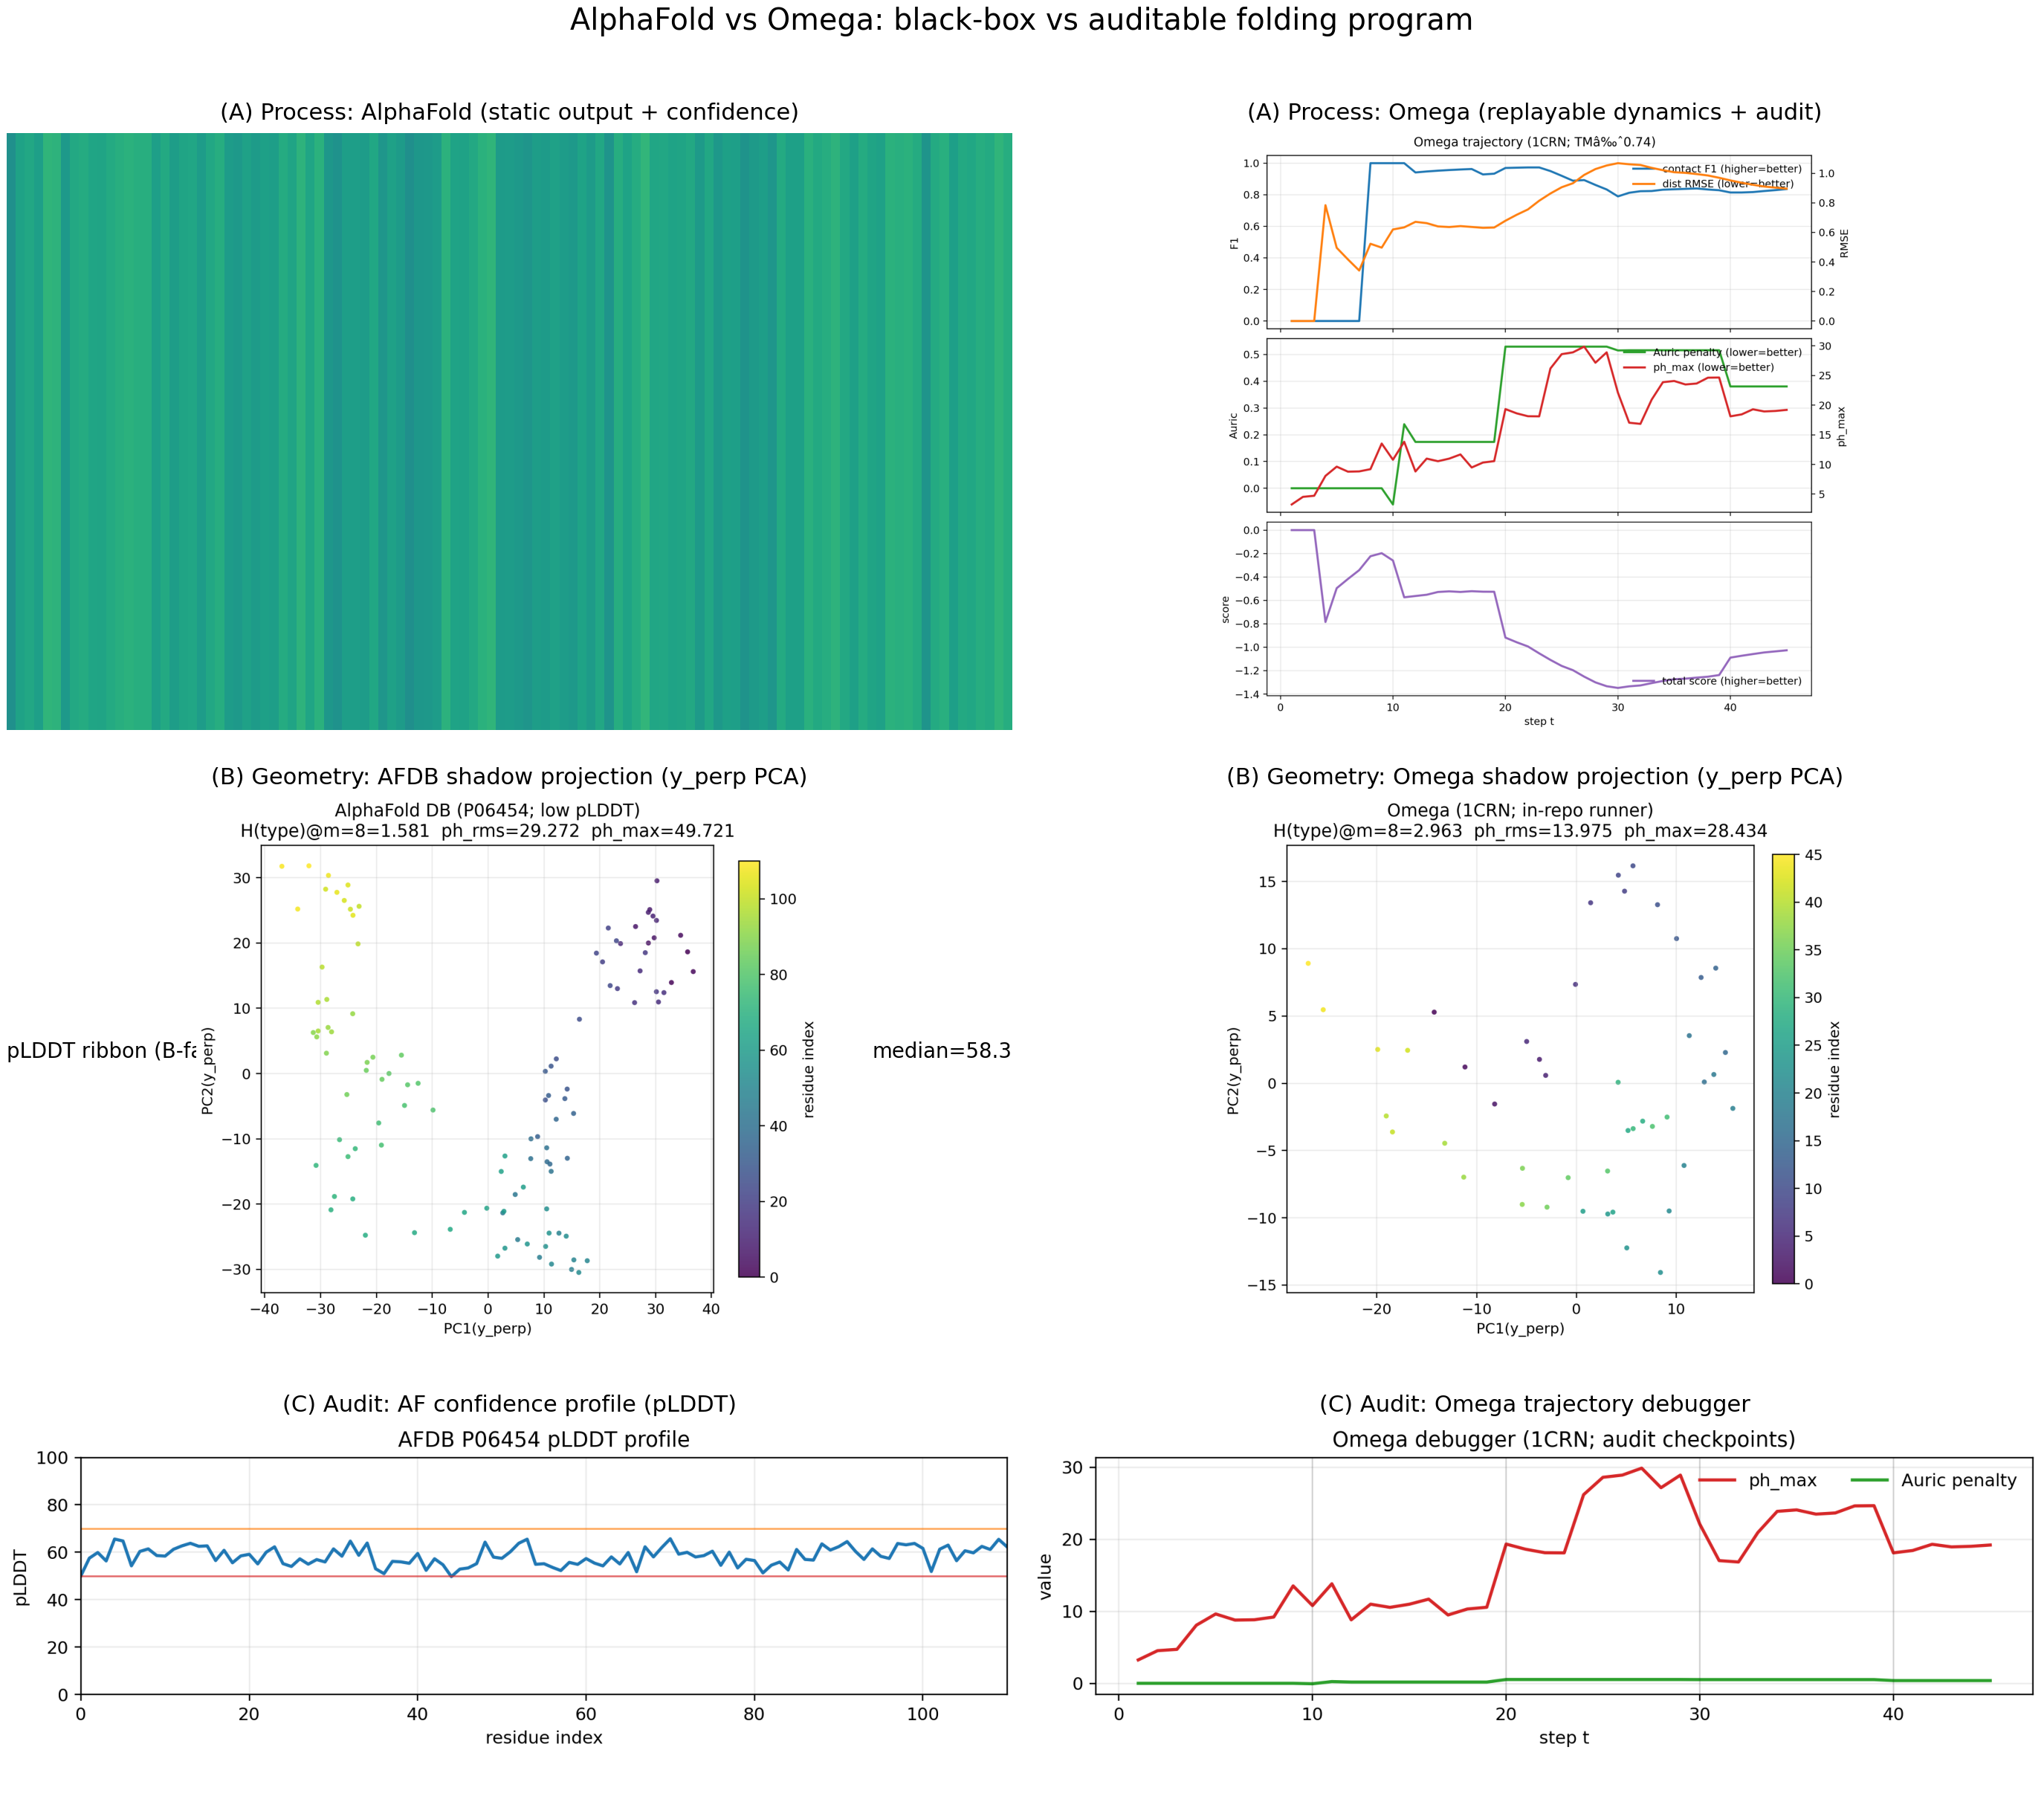
\includegraphics[width=\linewidth]{assets/figures/fig_af_vs_omega.png}
  \caption{\textbf{AlphaFold vs PhasonFold: black-box output vs replayable, auditable dynamics.}
  \textbf{(A) Process:} AlphaFold DB provides a static structure estimate and a per-residue confidence profile (pLDDT), while PhasonFold exposes an explicit, replayable trajectory with logged objective terms and audit readouts.
  \textbf{(B) Geometry:} a ``shadow projection'' of the perpendicular-space trace ($y_\perp$ PCA) highlights a qualitative difference between an AFDB low-confidence intrinsically disordered example (UniProt P06454) and a PhasonFold reconstruction example (1CRN) under the same 6D lifting/quantization protocol.
  \textbf{(C) Audit/debugger:} AlphaFold exposes confidence as an output-side annotation, whereas PhasonFold exposes an internal audit signal (phason proxy and checkpoint diagnostics) that supports targeted interventions and operator-level A/B tests.
  All run artifacts used to build this figure are provided in the accompanying evidence repository. As a robustness check against ``hand-picked IDP'' criticism, we also include a second AFDB example with mixed-confidence regions (UniProt P04637; p53).}
  \label{fig:af_vs_omega_transparency}
\end{figure}

First, low-resolution objectives are sufficient to drive search to apparently high-quality solutions, but they can also hide off-manifold failures. This motivates a principled separation between optimized readouts and audit-only residuals, and it provides a natural testbed for mechanistic gates.

Second, phason is most useful when treated as a dynamical feasibility variable rather than a static filter. In biophysical terms, tight perpendicular-space gates act like \emph{hard constraints} that can become effectively unsatisfiable under limited representational expressivity (alphabet coarseness) or a misaligned slice offset. Feasible-tight regimes ($\theta^\star$) therefore highlight the role of projector-style repair: without repair, hard rejection can freeze exploration; with repair (small $\Delta w_0$ updates), the constraint becomes an actionable relaxation mechanism that maintains sampling while enforcing manifold adherence.

Third, representational expressivity is a hard ceiling. The Triple232 alphabet reveals that TM-score >0.9 is attainable within the 6D framework, and the Sprint-to-0.9 results show that combining hotspot expressivity with piecewise phason repair can cross that threshold on long-chain and membrane-protein targets.

\paragraph{Orthogonality of certificates.}
Our decoy benchmarks reveal a functional dichotomy between two binary readouts. The geometry-based $\rho_A$ (perpendicular-space order) provides strong discrimination against hard-negative decoys (which are physically plausible but geometrically incorrect), whereas the logic/dynamics readout $\rho_B$ (step parity/velocity) provides weaker separation on hard decoys but excels at distinguishing random and shuffled nulls. This suggests an orthogonal defense mechanism: $\rho_B$ filters out non-computational random walks, while $\rho_A$ enforces specific geometric manifold constraints on the remaining plausible folds.

\paragraph{The ``Geometric Trap'' phenomenon in blind search.}
The Blind Sprint ablation highlights a protocol-sensitive failure mode on \texttt{3ICB}: enforcing $\rho_A$ (geometry) during the early search phase can be too restrictive, trapping the agent in basins that are geometrically feasible under the 6D projection but topologically incorrect (TM drops to $\approx$0.22 in best-of-seeds). In contrast, the logic/dynamics certificate $\rho_B$ (parity/velocity) maintains or improves performance on the same target, consistent with a softer dynamical consistency check that preserves traversal across barriers in the search landscape. This motivates a practical division of labor: use $\rho_B$ as the primary guidance term to maximize acceptance rate in blind search, and apply $\rho_A$ post-hoc as a stricter geometric auditor and hard-negative discriminator.

\paragraph{Physics audit layer as a low-cost ``witness''.}
Because our current experiments are C$\alpha$-only and geometry-driven, a natural reviewer concern is whether certificate-feasible structures are also physically plausible. Without changing the search objective, we therefore add a post-hoc ``physics audit layer'' based on fast CA-level proxies (bond-length MSE and a non-neighbour steric clash proxy), summarized as a single normalized physics score (clashes/$N$ + 1000$\times$bond MSE). On a realistic hard-negative benchmark (Decoys 'R' Us \texttt{4state\_reduced}), the physics score and the geometry-based certificate are weakly correlated (Fig.~S\ref{fig:physics_audit}; Pearson $r\approx 0$), yielding a \textbf{dual-filter} interpretation: many decoys remain locally physical while violating global manifold constraints (high geometric type entropy), while a smaller subset exhibits the converse (low geometric type entropy but poor local physics). This motivates an orthogonal defense mechanism: the geometric certificate filters ``physically plausible but geometrically invalid'' conformations, while the physics audit catches gross local crowding before any expensive full-atom refinement. As a stronger complement, the coordinate-constrained Rosetta relaxation audit (Fig.~\ref{fig:5}) shows that the C$\alpha$ backbones also occupy stable basins under a standard all-atom energy function.


Limitations remain substantial. Current experiments are C$\alpha$-only and target-conditioned (they reconstruct known structures rather than predict from sequence alone). The phason window model is approximate and will require a more faithful acceptance domain and improved lift definitions. Importantly, in a 1000-structure PDB survey using operational phason proxies (global mean, piecewise, and linear-drift-corrected centering), real backbones do not show a strong, uniform separation from simple matched random-chain controls; this suggests that a ``low-phason submanifold'' should be treated as a testable hypothesis rather than an established empirical fact under the present proxy/controls. We view this as a helpful distinction between \emph{satisfiability} (phason as a repairable constraint that makes hard regimes feasible, e.g. $\theta^\star$) and \emph{discriminability} (phason as a standalone detector of nativeness), and it motivates integrating stronger physics-facing objectives and controls. We also have not yet benchmarked against full-atom physics or contemporary end-to-end sequence predictors in a head-to-head setting. Nonetheless, the presented evidence supports a central claim: geometric priors can be compiled into executable, auditable dynamics, enabling mechanism-level A/B tests that are difficult to perform in continuous black-box pipelines.

Future work will focus on (i) semantic objectives (distograms/torsions) with physically grounded gates, (ii) multi-domain and polycrystalline piecewise slicing with learnable $w_0$ trajectories, (iii) membrane-aware packing constraints integrated directly into operator selection, and (iv) scaling to full domains (N>100) with hardware-friendly kernels.
